% ****** Start of file apssamp.tex ******
%
%   This file is part of the APS files in the REVTeX 4.1 distribution.
%   Version 4.1r of REVTeX, August 2010
%
%   Copyright (c) 2009, 2010 The American Physical Society.
%
%   See the REVTeX 4 README file for restrictions and more information.
%
% TeX'ing this file requires that you have AMS-LaTeX 2.0 installed
% as well as the rest of the prerequisites for REVTeX 4.1
%
% See the REVTeX 4 README file
% It also requires running BibTeX. The commands are as follows:
%
%  1)  latex apssamp.tex
%  2)  bibtex apssamp
%  3)  latex apssamp.tex
%  4)  latex apssamp.tex
%
\documentclass[%
 reprint,
%superscriptaddress,
%groupedaddress,
%unsortedaddress,
%runinaddress,
%frontmatterverbose, 
%preprint,
%showpacs,preprintnumbers,
%nofootinbib,
%nobibnotes,
%bibnotes,
 amsmath,amssymb,
 aps,
%pra,
%prb,
%rmp,
%prstab,
%prstper,
%floatfix,
]{revtex4-1}
\usepackage{fancyhdr}
\usepackage{todonotes}
\usepackage{hyperref}
\newcommand{\round}[1]{\ensuremath{\lfloor#1\rceil}}
\usepackage{epsfig} % for postscript graphics files
\usepackage{graphicx}% Include figure files
\usepackage{dcolumn}% Align table columns on decimal point
\usepackage{bm}% bold math
%\usepackage{hyperref}% add hypertext capabilities
%\usepackage[mathlines]{lineno}% Enable numbering of text and display math
%\linenumbers\relax % Commence numbering lines

%\usepackage[showframe,%Uncomment any one of the following lines to test 
%%scale=0.7, marginratio={1:1, 2:3}, ignoreall,% default settings
%%text={7in,10in},centering,
%%margin=1.5in,
%%total={6.5in,8.75in}, top=1.2in, left=0.9in, includefoot,
%%height=10in,a5paper,hmargin={3cm,0.8in},
%]{geometry}


\cfoot{\thepage}


\begin{document}
\title{{\LARGE \bf
Applications of Neural Networks to Facial Interpretation.}\newline {\small \bf Group 14}
}

%\author{ \parbox{3 in}{\centering Huibert Kwakernaak*
%         \thanks{*Use the $\backslash$thanks command to put information here}\\
%         Faculty of Electrical Engineering, Mathematics and Computer Science\\
%         University of Twente\\
%         7500 AE Enschede, The Netherlands\\
%         {\tt\small h.kwakernaak@autsubmit.com}}
%         \hspace*{ 0.5 in}
%         \parbox{3 in}{ \centering Pradeep Misra**
%         \thanks{**The footnote marks may be inserted manually}\\
%        Department of Electrical Engineering \\
%         Wright State University\\
%         Dayton, OH 45435, USA\\
%         {\tt\small pmisra@cs.wright.edu}}
%}
\author{J Mair,  O Hussein, B Foong, H Li and H Yuan% <-this % stops a space
}



\maketitle
\thispagestyle{empty}
\pagestyle{empty}


%%%%%%%%%%%%%%%%%%%%%%%%%%%%%%%%%%%%%%%%%%%%%%%%%%%%%%%%%%%%%%%%%%%%%%%%%%%%%%%%
%\begin{abstract}

%\par{We applied supervised learning techniques and neural networks to solve three problems based on labelled facial expression data. We first applied variants of the K-Nearest Neighbour (KNN) algorithm to provide a baseline for our results. We used 10 fold cross validation to produce results from each neural network. We managed to train a neural network on the binary smile/no smile data set to achieve a mean accuracy of (87$\pm$15)\%. The second problem was emotion classification and we achieved a mean accuracy of (73$\pm$6)\%. In the final regression problem we achieved a mean square error of \todo[inline]{inset here}.}

%\end{abstract}


%%%%%%%%%%%%%%%%%%%%%%%%%%%%%%%%%%%%%%%%%%%%%%%%%%%%%%%%%%%%%%%%%%%%%%%%%%%%%%%%
\section{Introduction}


\section{Method}

\subsection{Preprocessing}
\par{We processed each feature set into a 2D array in which each column represents a single sample of features. In the case of the binary and regression data this involved reshaping the two spacial dimensions of each facial point into a single dimension.}
\par{For the multi-class label set we needed to convert each category label (integer values of 1 to 6) into "One-Hot Encoding"\cite{feml}, due to it allowing a better description of an error function. The error function we can use therefore is cross-entropy which allows us to qualify definitive predictions as better, which is expected to increase the generalisation ability of a network. The original integer makes the output orderable orderable\cite{feml}, which is unexpressive for classification problems.}
\par{From the regression data set we extracted the 6$^{th}$ label from each sample which represented the yaw of the head.}
\par{Finally we produced a random permutation of each data and label set pair to allow random train/test split of the data in our experiments. This was done using a seeded random number generator so that the results were repeatable.}

\subsection{K-Nearest Neighbour Tests}

\par{As a baseline, we applied variants of the K-Nearest Neighbour (KNN) algorithm to each different data set. On the two classification problems, we cross validated the KNN algorithm with 4 folds and plotted a confusion matrix as seen in \autoref{fig:knn_bin} and \autoref{fig:knn_multi}. These gained accuracies of (81$\pm$6)\% and (54$\pm$4)\% for the binary and mutli-class problem respectively, averaged across a 4 fold cross-validation set.}
\par{For the regression problem we slightly altered the KNN algorithm so that it would take the mean of the k nearest labels instead of the mode, due to the continuous nature of the output. This algorithm was used with k=3 and 4 fold cross-validation to obtain root mean square error as $1.8\pm0.3$.}

\begin{figure}
    \centering
    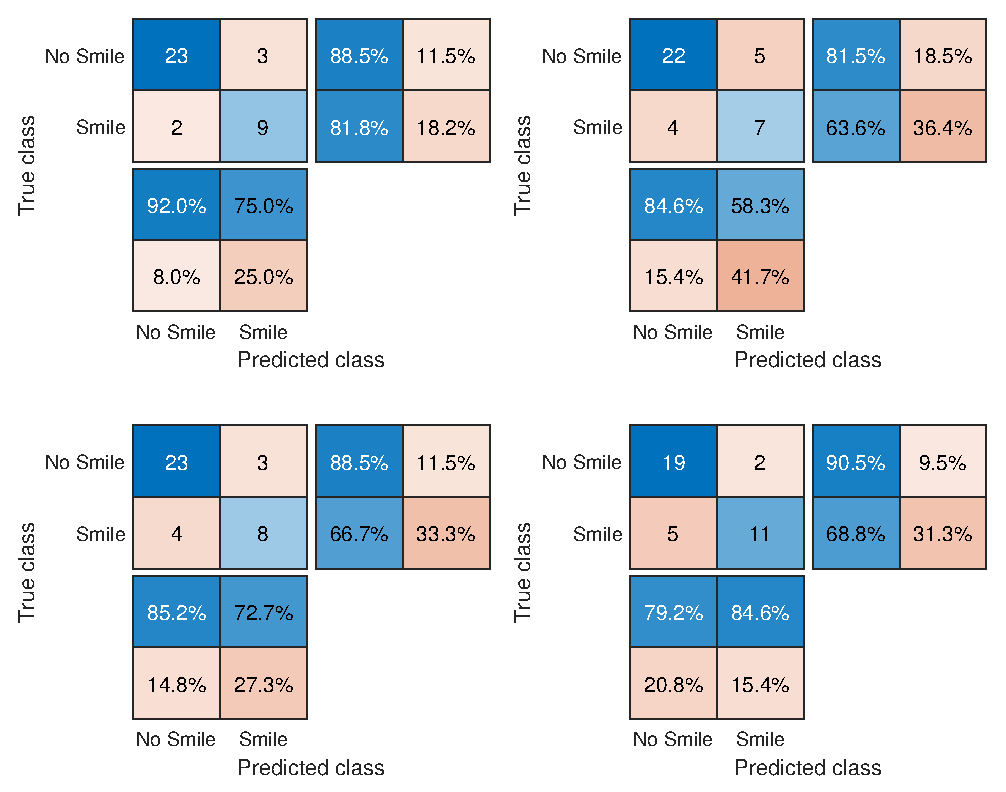
\includegraphics[width=0.45\textwidth]{binaryknn.eps}
    \caption{Classification results for the KNN algorithm (k=3) on the binary problem with 4 fold cross-validation. This algorithm got a mean F1 score of 0.86$\pm$0.03 for class 0 (not smile) and 0.71$\pm$0.08.}
    \label{fig:knn_bin}
\end{figure}

\begin{figure}
    \centering
    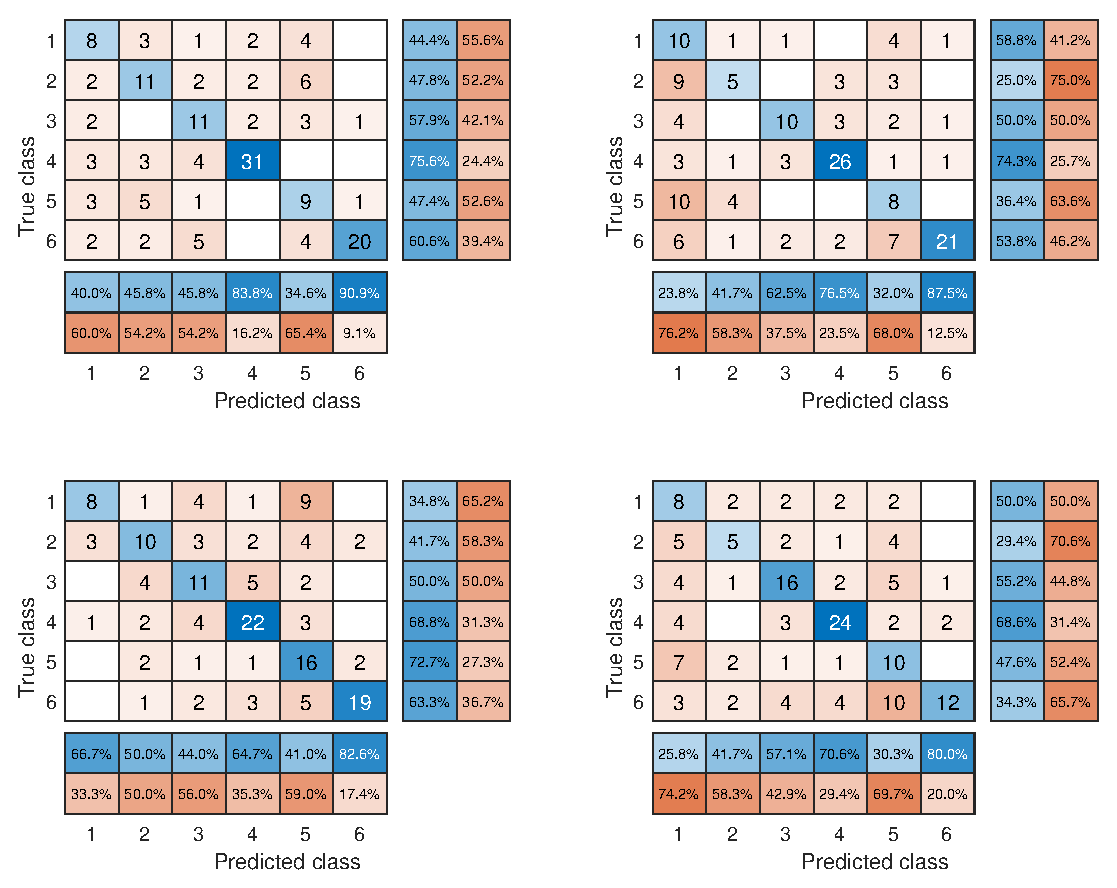
\includegraphics[width=0.45\textwidth]{multiknn.eps}
    \caption{Classification results for the KNN algorithm (k=5) on the multiclass problem with 4 fold cross-validation. This algorithm got mean F1 scores of 0.39, 0.40, 0.52, 0.73, 0.41 and 0.65 for the classes 1 to 6 respectively.}
    \label{fig:knn_multi}
\end{figure}

\subsection{Neural Networks}

\subsubsection{Binary Classification}

\par{Upon inspecting this data set we noticed that the distribution of classes was weighted towards the "No Smile" class. We tried to avoid biasing the network and as a result we choose the network topology and hyper parameters that resulted in better F1 scores, since the accuracy would not be enough.}
\par{In training we used the mean square error as a performance measure and so we reasoned that the network would make predicts close to 0 or 1. To make a decision we used the following formula:
\begin{equation}
Y_i = \round{\max(0, \min(y_i, 1))}
\end{equation}
, where $Y_i$ is the actual prediction and $y_i$ is the output from the network.}
\par{Upon training we decided on a simple network topology and hyper parameters, which is shown in \autoref{fig:nn_bin}, since our data set was extremely small. We tried to minimise the number of intrinsic parameter to avoid over-fitting; this included adding early stopping mechanisms by changing the number of epochs and validation checks to a smaller number.}

\begin{figure}
    \centering
    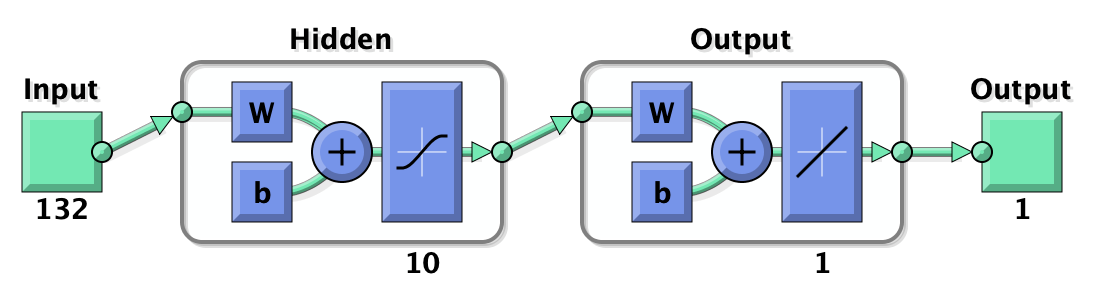
\includegraphics[width=0.45\textwidth]{binarytopology.png}
    \caption{Network topology for the binary neural network. This was trained using Bayesian regularization backpropagation\cite{trainbr}, epochs set to 100 and the Marquardt adjustment parameter set to 0.005.}
    \label{fig:nn_bin}
\end{figure}

\par{Training this network resulted in a mean F1 score of 0.92 for class 0 (not smile) and 0.86 for class 1 (smile) and a mean accuracy of (91$\pm$2)\% across the 10 fold cross-validation sets.}

\begin{figure}
    \centering
    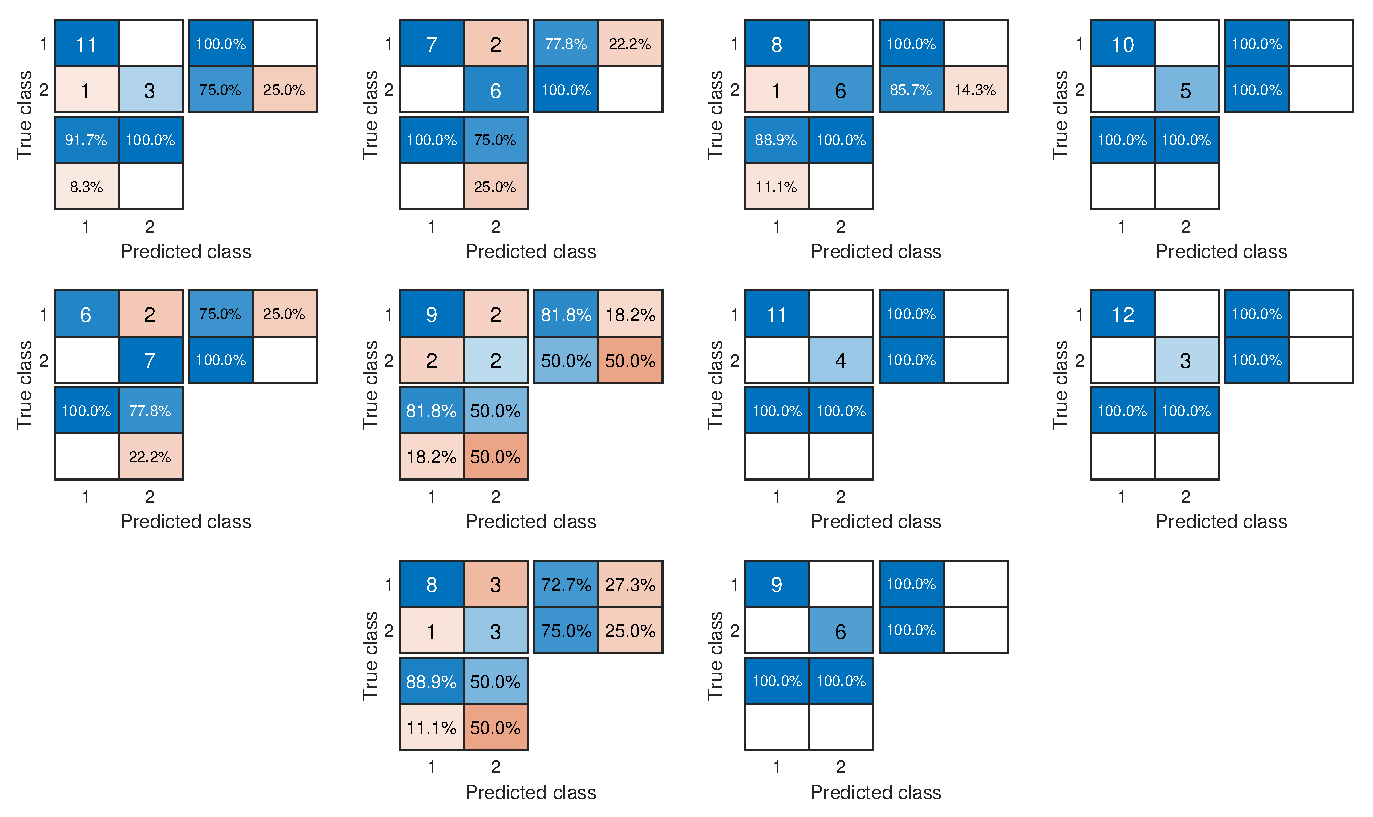
\includegraphics[width=0.45\textwidth]{binarynn.eps}
    \caption{The confusion matrices for each different cross validation upon training the network in \autoref{fig:nn_bin}.}
    \label{fig:nn_bin_results}
\end{figure}

\subsubsection{Multi-class Classification}



\par{After receiving the preprocessed data from earlier, we experimented with different training mechanisms. At first we used the default \textit{feedforwardnet} supplied in the MATLAB toolbox\cite{dltoolbox}, however we compared it to using \textit{patternnet} instead and found that this performed better on F1 scores from the confusion matrix.}


\begin{figure}
    \centering
    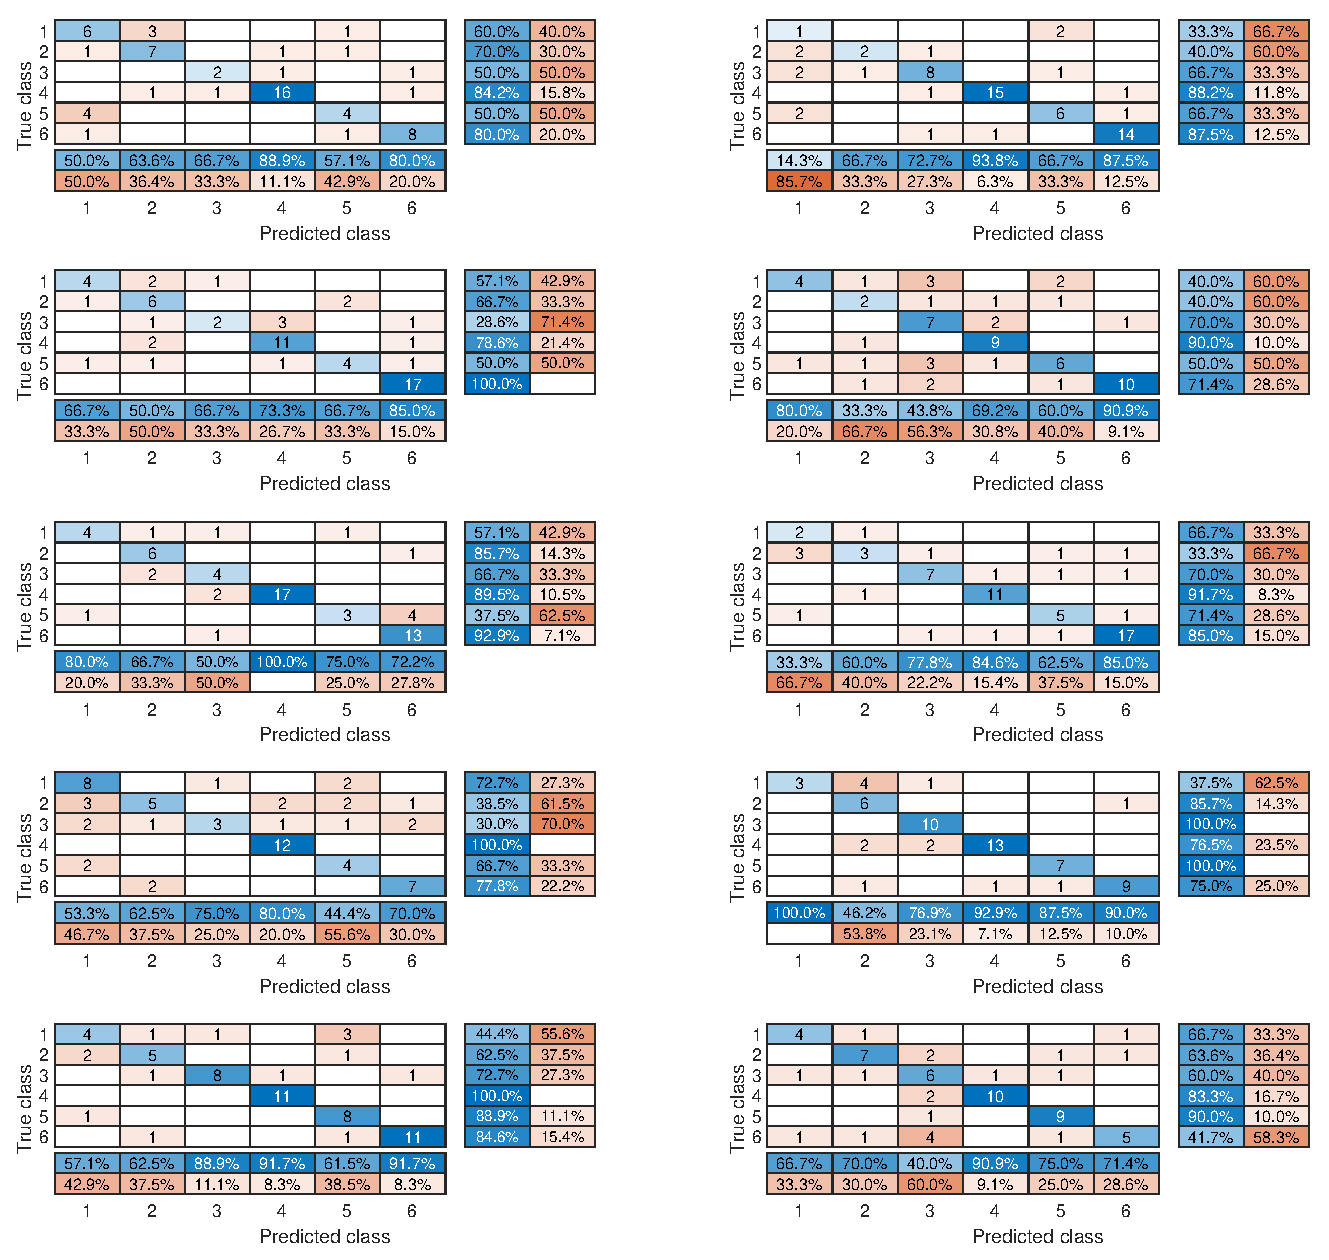
\includegraphics[width=0.5\textwidth,height=0.8\textwidth]{multicrossvalidationconfusionmatrices.eps}
    \caption{The confusion matrices yielded from each of the 10 cross validation sets.}
    \label{fig:nn_multi_results}
\end{figure}
\par{We attempted to use meta optimisation on this problem but found that the data set was far too small and any major meta optimisation would result in over fitting and a biased value of the mean. Instead we stopped our tests early and picked a set of parameters that achieved an average classification accuracy of (70$\pm$6)\%. This network architecture is shown in \autoref{fig:nn_multi}.}

\begin{figure}
    \centering
    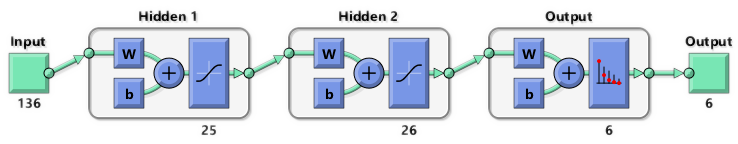
\includegraphics[width=0.45\textwidth]{multitopology1.png}
    \caption{Network topology for the multi-class neural network. This was trained using Scaled conjugate gradient backpropagation\cite{trainscg}, with sigma set to 0.00036915, lambda set to 0.00025801, epochs set to 500 and max fail set to 10.}
    \label{fig:nn_multi}
\end{figure}

\par{Our results yielded a mean confusion matrix as shown in \autoref{fig:nn_multi_results} and F1 result over all classes and cross validation set of 0.56, 0.58, 0.62, 0.86, 0.72 and 0.81 for the classes 1 to 6 respectively. This yielded an accuracy of (73$\pm$6)\%.}


\subsubsection{Regression}

\par{For our final set we tried a few network structures. Despite some success with the two classification models, our attempts to manually adjust our hyper-parameters to achieve a MSE below the KNN results were futile. We therefore used a hyper heuristic to tune our hyper parameters. Our aim was to minimise the average MSE under cross-validation. If we were to simply apply this to our entire data set we would be at risk of over fitting to our sample data. To avoid this we randomly split the data set having 40\% to try and find more optimal hyper-parameters and leaving 60\% to do a final cross validation check on the provided settings.}
\par{The hyper heuristic used was the bayesopt\cite{bayesopt} function. This function was allowed to alter the topology of the network (the number of neurons in each of the 4 hidden layers) while also changing two of the hyper parameters of the learning function\cite{trainlm}. The hyper heuristic selected the topology and hyper parameters shown in \autoref{fig:nn_reg}.}
\par{These parameters were used structure and train a neural network to which got an average root mean square error of 1.8$\pm$0.3.}

\begin{figure}
    \centering
    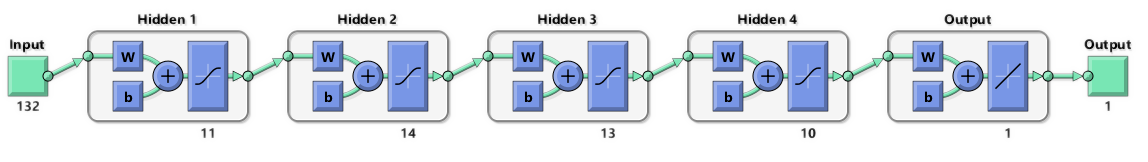
\includegraphics[width=0.5\textwidth]{regresstopology1.png}
    \caption{Network topology for the regression neural network. This was trained using Levenberg-Marquardt backpropagation\cite{trainlm} with epochs set to 500, max fail at 5, mu at 69.242 and minimum gradient set to 2.3122. All other settings were at their default.}
    \label{fig:nn_reg}
\end{figure}

\section{Conclusions}

%%%%%%%%%%%%%%%%%%%%%%%%%%%%%%%%%%%%%%%%%%%%%%%%%%%%%%%%%%%%%%%%%%%%%%%%%%%%%%%%

\bibliography{references}

\bibliographystyle{unsrt}



\end{document}
